% Options for packages loaded elsewhere
% Options for packages loaded elsewhere
\PassOptionsToPackage{unicode}{hyperref}
\PassOptionsToPackage{hyphens}{url}
\PassOptionsToPackage{dvipsnames,svgnames,x11names}{xcolor}
%
\documentclass[
]{article}
\usepackage{xcolor}
\usepackage{amsmath,amssymb}
\setcounter{secnumdepth}{5}
\usepackage{iftex}
\ifPDFTeX
  \usepackage[T1]{fontenc}
  \usepackage[utf8]{inputenc}
  \usepackage{textcomp} % provide euro and other symbols
\else % if luatex or xetex
  \usepackage{unicode-math} % this also loads fontspec
  \defaultfontfeatures{Scale=MatchLowercase}
  \defaultfontfeatures[\rmfamily]{Ligatures=TeX,Scale=1}
\fi
\usepackage{lmodern}
\ifPDFTeX\else
  % xetex/luatex font selection
\fi
% Use upquote if available, for straight quotes in verbatim environments
\IfFileExists{upquote.sty}{\usepackage{upquote}}{}
\IfFileExists{microtype.sty}{% use microtype if available
  \usepackage[]{microtype}
  \UseMicrotypeSet[protrusion]{basicmath} % disable protrusion for tt fonts
}{}
\makeatletter
\@ifundefined{KOMAClassName}{% if non-KOMA class
  \IfFileExists{parskip.sty}{%
    \usepackage{parskip}
  }{% else
    \setlength{\parindent}{0pt}
    \setlength{\parskip}{6pt plus 2pt minus 1pt}}
}{% if KOMA class
  \KOMAoptions{parskip=half}}
\makeatother
% Make \paragraph and \subparagraph free-standing
\makeatletter
\ifx\paragraph\undefined\else
  \let\oldparagraph\paragraph
  \renewcommand{\paragraph}{
    \@ifstar
      \xxxParagraphStar
      \xxxParagraphNoStar
  }
  \newcommand{\xxxParagraphStar}[1]{\oldparagraph*{#1}\mbox{}}
  \newcommand{\xxxParagraphNoStar}[1]{\oldparagraph{#1}\mbox{}}
\fi
\ifx\subparagraph\undefined\else
  \let\oldsubparagraph\subparagraph
  \renewcommand{\subparagraph}{
    \@ifstar
      \xxxSubParagraphStar
      \xxxSubParagraphNoStar
  }
  \newcommand{\xxxSubParagraphStar}[1]{\oldsubparagraph*{#1}\mbox{}}
  \newcommand{\xxxSubParagraphNoStar}[1]{\oldsubparagraph{#1}\mbox{}}
\fi
\makeatother


\usepackage{longtable,booktabs,array}
\usepackage{calc} % for calculating minipage widths
% Correct order of tables after \paragraph or \subparagraph
\usepackage{etoolbox}
\makeatletter
\patchcmd\longtable{\par}{\if@noskipsec\mbox{}\fi\par}{}{}
\makeatother
% Allow footnotes in longtable head/foot
\IfFileExists{footnotehyper.sty}{\usepackage{footnotehyper}}{\usepackage{footnote}}
\makesavenoteenv{longtable}
\usepackage{graphicx}
\makeatletter
\newsavebox\pandoc@box
\newcommand*\pandocbounded[1]{% scales image to fit in text height/width
  \sbox\pandoc@box{#1}%
  \Gscale@div\@tempa{\textheight}{\dimexpr\ht\pandoc@box+\dp\pandoc@box\relax}%
  \Gscale@div\@tempb{\linewidth}{\wd\pandoc@box}%
  \ifdim\@tempb\p@<\@tempa\p@\let\@tempa\@tempb\fi% select the smaller of both
  \ifdim\@tempa\p@<\p@\scalebox{\@tempa}{\usebox\pandoc@box}%
  \else\usebox{\pandoc@box}%
  \fi%
}
% Set default figure placement to htbp
\def\fps@figure{htbp}
\makeatother


% definitions for citeproc citations
\NewDocumentCommand\citeproctext{}{}
\NewDocumentCommand\citeproc{mm}{%
  \begingroup\def\citeproctext{#2}\cite{#1}\endgroup}
\makeatletter
 % allow citations to break across lines
 \let\@cite@ofmt\@firstofone
 % avoid brackets around text for \cite:
 \def\@biblabel#1{}
 \def\@cite#1#2{{#1\if@tempswa , #2\fi}}
\makeatother
\newlength{\cslhangindent}
\setlength{\cslhangindent}{1.5em}
\newlength{\csllabelwidth}
\setlength{\csllabelwidth}{3em}
\newenvironment{CSLReferences}[2] % #1 hanging-indent, #2 entry-spacing
 {\begin{list}{}{%
  \setlength{\itemindent}{0pt}
  \setlength{\leftmargin}{0pt}
  \setlength{\parsep}{0pt}
  % turn on hanging indent if param 1 is 1
  \ifodd #1
   \setlength{\leftmargin}{\cslhangindent}
   \setlength{\itemindent}{-1\cslhangindent}
  \fi
  % set entry spacing
  \setlength{\itemsep}{#2\baselineskip}}}
 {\end{list}}
\usepackage{calc}
\newcommand{\CSLBlock}[1]{\hfill\break\parbox[t]{\linewidth}{\strut\ignorespaces#1\strut}}
\newcommand{\CSLLeftMargin}[1]{\parbox[t]{\csllabelwidth}{\strut#1\strut}}
\newcommand{\CSLRightInline}[1]{\parbox[t]{\linewidth - \csllabelwidth}{\strut#1\strut}}
\newcommand{\CSLIndent}[1]{\hspace{\cslhangindent}#1}



\setlength{\emergencystretch}{3em} % prevent overfull lines

\providecommand{\tightlist}{%
  \setlength{\itemsep}{0pt}\setlength{\parskip}{0pt}}



 


\makeatletter
\@ifpackageloaded{caption}{}{\usepackage{caption}}
\AtBeginDocument{%
\ifdefined\contentsname
  \renewcommand*\contentsname{Table of contents}
\else
  \newcommand\contentsname{Table of contents}
\fi
\ifdefined\listfigurename
  \renewcommand*\listfigurename{List of Figures}
\else
  \newcommand\listfigurename{List of Figures}
\fi
\ifdefined\listtablename
  \renewcommand*\listtablename{List of Tables}
\else
  \newcommand\listtablename{List of Tables}
\fi
\ifdefined\figurename
  \renewcommand*\figurename{Figure}
\else
  \newcommand\figurename{Figure}
\fi
\ifdefined\tablename
  \renewcommand*\tablename{Table}
\else
  \newcommand\tablename{Table}
\fi
}
\@ifpackageloaded{float}{}{\usepackage{float}}
\floatstyle{ruled}
\@ifundefined{c@chapter}{\newfloat{codelisting}{h}{lop}}{\newfloat{codelisting}{h}{lop}[chapter]}
\floatname{codelisting}{Listing}
\newcommand*\listoflistings{\listof{codelisting}{List of Listings}}
\makeatother
\makeatletter
\makeatother
\makeatletter
\@ifpackageloaded{caption}{}{\usepackage{caption}}
\@ifpackageloaded{subcaption}{}{\usepackage{subcaption}}
\makeatother
\usepackage{bookmark}
\IfFileExists{xurl.sty}{\usepackage{xurl}}{} % add URL line breaks if available
\urlstyle{same}
\hypersetup{
  pdftitle={Methods for Reconstructing Paleo Food Webs},
  pdfauthor={Tanya Strydom; Andrew P. Beckerman},
  pdfkeywords={food web, network construction},
  colorlinks=true,
  linkcolor={blue},
  filecolor={Maroon},
  citecolor={Blue},
  urlcolor={Blue},
  pdfcreator={LaTeX via pandoc}}



\title{Methods for Reconstructing Paleo Food Webs}
\author{Tanya Strydom %
%
\textsuperscript{%
%
1%
}%
; Andrew P. Beckerman %
%
\textsuperscript{%
%
1%
}%
}
\date{2025-06-30}

\usepackage{setspace}
\usepackage[left]{lineno}
\usepackage[letterpaper]{geometry}

\usepackage[nolists,noheads,markers]{endfloat}
\geometry{margin=2.5cm}

\begin{document}

\thispagestyle{empty}
{\bfseries\sffamily\Large Methods for Reconstructing Paleo Food Webs}
\vfil
Tanya Strydom %
%
\textsuperscript{%
%
1%
}%
; Andrew P. Beckerman %
%
\textsuperscript{%
%
1%
}%

\vfil
{\small
\textbf{Abstract:} Food webs represent the feeding relationships between
species and can help infer ecosystem-level processes. Alongside the
development of food web theory, methods for constructing food webs have
been developed to infer species interactions when empirical data is
lacking. Food web construction methods are diverse, each utilising
different approaches to infer species interactions ---such as the use of
traits to infer mechanistic relationships vs using gut content as a
proxy for species diets. These methods have distinct theories,
mechanisms, and data requirements. In paleoecology, where direct
evidence of feeding interactions are rare, food web construction methods
are especially valuable and affords us the opportunity to make
inferences about paleo communities beyond simply a record of species
composition. However, the limitations of paleontological data (e.g.,
information of species traits is limited to that which can be preserved)
restrict which methods can reliably be used. By considering both
ecological theory and the constraints of what can be derived from the
fossil record, we identify the methods best suited for the construction
of paleo food webs. Specifically, we focus on how these methods differ
in the networks they produce and what these networks can reveal about
species interactions. In doing so we hope to clarify the ecological
nuances of network prediction and help prevent the accidental misuse or
misinterpretation of paleo food webs.
\vfil
\textbf{Keywords:} %
food web, %
network construction%
}
\clearpage
\setcounter{page}{1}
\doublespacing
\linenumbers


\section{Why build paleo food webs?}\label{why-build-paleo-food-webs}

\begin{itemize}
\item
  Because its interesting? Point to works that showcase how we can learn
  form the past and inform on the current but possibly also the future
\item
  Value in using hindcasting to aid in forecasting. \emph{e.g.,} the
  Toarcian ms (Dunhill et al., 2024) shows how we can use these paleo
  communities to understand trophic-level responses to extinctions.
\item
  Close out with the inherit challenge that we cannot observe paleo
  feeding interactions (barring rare instances, and often only for a
  limited subset of species) and so we are often using expert
  knowledge/mechanistic assumptions to infer links between species
  (*e.g.,* Dunne et al., 2014; Roopnarine, 2006).
\end{itemize}

\section{How do we build paleo food
webs?}\label{how-do-we-build-paleo-food-webs}

\begin{itemize}
\item
  There is an evolving body of work that focuses on developing tools
  specifically for the task of predicting food webs.
\item
  There are a handful that have been developed specifically in the
  context of paleo settings (Fricke et al., 2022; Roopnarine, 2006;
  *e.g.,* Shaw et al., 2024) but we can also talk about those that might
  have been developed/tested in contemporary settings but still have
  applicability in paleo ones.
\item
  Different underlying theory though

  \begin{itemize}
  \tightlist
  \item
    Focus here on the idea of different `currencies' but also
    aggregations - energy vs compatibility.
  \end{itemize}
\item
  Insert brief overview of the different methods as they pertain to
  approach (so the T4T triangle)
\item
  Challenges we face (even in contemporary settings)?

  \begin{itemize}
  \tightlist
  \item
    keep high level - I think the argument here should fall more in the
    data trade offs\ldots{}
  \end{itemize}
\end{itemize}

\section{Understanding how networks are
different}\label{understanding-how-networks-are-different}

It is important to be aware that networks can be configured in different
ways depending on how the interactions are defined (Strydom, in prep).
Basically we have metawebs (which represent \emph{potential}
interactions), realised networks (which represent the subset of
potential that are realised as a result of community and environmental
context), and structural networks (species agnostic networks that are
structurally informative). Here also talk about the implications of
these different networks types - different uses and capturing different
processes. Speciifcally link this to models - \emph{i.e.,} different
models have been developed to construct a \emph{specific} network
representation.

\section{Challenges specific to building paleo
communities/networks}\label{challenges-specific-to-building-paleo-communitiesnetworks}

Although there has been a push for the development of tools and methods
that allow us to predict species interactions and networks {[}see
\emph{e.g.,} XXX for some reviews{]} they will not all be suitable for
the prediction of paleo communities. This is primarily due to
limitations that we are faced with in terms of the information that can
be inferred from the fossil record (such as species traits abundances,
and assemblages), which is needed as input data for the different
models. The limited information available from the fossil record is
compounded by the incomplete and biased preservation of species
{[}REF{]}, the spatial ambiguity of fossils found in a location {[}were
species conserved \emph{in situ} or were they there owing to geological
processes; REF{]}, and an increasing degree of `fuzziness' the further
one moves back in geological time {[}our understanding of both
phylogenetic and functional trait space, REF{]}. Methodologically
speaking some tools that `learn' from contemporary communities
(\emph{e.g.,} Strydom et al. (2023), Caron et al. (2022)) will become
`worse' the further one goes back in time since species then look very
different from now but can still be useful for `recent' communities
(\emph{e.g.,} Fricke et al. (2022)). This is not to say that it is
impossible to construct paleo networks but rather identify that there
are a subset of models that are probably not at all suitable for
constructing paleo networks (\emph{e.g.,} Null models, since there are
fully driven by abundance), other methods will be better suited
depending on the community of interest \emph{e.g.,} for more
contemporary communities that have modern analogs we can use methods
rooted in phylogeny (\emph{e.g.,} Fricke et al. (2022), Strydom et al.
(2023)) or traits (\emph{e.g.,} Caron et al. (2022)), and then there is
the third axis which is to think about which are the assumptions that
are made and there trade off of that. This includes thinking about both
assumptions you are making about the actual data \emph{e.g.,} trying to
extrapolate body size from fossil data but also assumptions across time
\emph{e.g.,} assuming modern trait-feeding modes are the same OR that
assumptions about network structure will hold across deep time.

\section{Approaches to food web
prediction}\label{approaches-to-food-web-prediction}

Here we should take the time to go in and just articulate that there are
nuance and differences in terms of predicting interactions vs predicting
networks. Once it is finally on a preprint server we can obviously link
to the T4T stuff\ldots{}

Here we present six different models (Table~\ref{tbl-models}) that can
be used to construct food webs for both this specific community but are
also broadly suited to paleo network prediction. These models span all
facets of the network representation space (metaweb, realised, and
structural network) and are suitable for an array of different paleo
communities as the data requirements are `paleo friendly'.

\begin{longtable}[]{@{}
  >{\raggedright\arraybackslash}p{(\linewidth - 10\tabcolsep) * \real{0.1667}}
  >{\raggedright\arraybackslash}p{(\linewidth - 10\tabcolsep) * \real{0.1667}}
  >{\raggedright\arraybackslash}p{(\linewidth - 10\tabcolsep) * \real{0.1667}}
  >{\raggedright\arraybackslash}p{(\linewidth - 10\tabcolsep) * \real{0.1667}}
  >{\raggedright\arraybackslash}p{(\linewidth - 10\tabcolsep) * \real{0.1667}}
  >{\raggedright\arraybackslash}p{(\linewidth - 10\tabcolsep) * \real{0.1667}}@{}}
\caption{A summary of the different families of tools that can be used
to generate paleo food webs.}\label{tbl-models}\tabularnewline
\toprule\noalign{}
\begin{minipage}[b]{\linewidth}\raggedright
Model family
\end{minipage} & \begin{minipage}[b]{\linewidth}\raggedright
Assumptions
\end{minipage} & \begin{minipage}[b]{\linewidth}\raggedright
Data needs
\end{minipage} & \begin{minipage}[b]{\linewidth}\raggedright
`Limitation'
\end{minipage} & \begin{minipage}[b]{\linewidth}\raggedright
Network type
\end{minipage} & \begin{minipage}[b]{\linewidth}\raggedright
Key reference
\end{minipage} \\
\midrule\noalign{}
\endfirsthead
\toprule\noalign{}
\begin{minipage}[b]{\linewidth}\raggedright
Model family
\end{minipage} & \begin{minipage}[b]{\linewidth}\raggedright
Assumptions
\end{minipage} & \begin{minipage}[b]{\linewidth}\raggedright
Data needs
\end{minipage} & \begin{minipage}[b]{\linewidth}\raggedright
`Limitation'
\end{minipage} & \begin{minipage}[b]{\linewidth}\raggedright
Network type
\end{minipage} & \begin{minipage}[b]{\linewidth}\raggedright
Key reference
\end{minipage} \\
\midrule\noalign{}
\endhead
\bottomrule\noalign{}
\endlastfoot
random & Links are randomly distributed within a network & richness,
number of links & parameter assumptions, species agnostic & structural
network & Erdős \& Rényi (1959) \\
niche & Networks are interval, species can be ordered on a `niche axis'
& richness, connectance & parameter assumptions, species agnostic &
structural network & Williams \& Martinez (2008) \\
allometric diet breadth model (ADBM) & Interactions are determined by
energetic costs (foraging ecology) & body mass, biomass (abundance) &
does not account for forbidden links in terms of trait compatibility,
assumptions on body size and biomass (abundance) from fossil data &
realised network & Petchey et al. (2008) \\
l-matrix & Interactions inferred using allometric rules (ratio of body
sizes between predator and prey), with links being constrained by a
Ricker function & body mass, number of producer species & does not
account for forbidden links in terms of trait compatibility, assumptions
on body size from fossil data, assumptions as to the number of producer
species & realised network & Schneider et al. (2016) \\
paleo food web inference model (PFIM) & Interactions can be inferred by
a mechanistic framework/relationships & feeding traits for taxa,
mechanistic feeding rules & Assumption made as to the feeding
mechanisms, need to elucidate traits from models (although this is a way
smaller issue) & metaweb & Shaw et al. (2024) \\
body size ratio model & Interactions inferred using allometric rules
(ratio of body sizes between predator and prey). :ogit of the linking
probability used to further constrain links to an `optimal size range'
for prey. & body mass & does not account for forbidden links in terms of
evolutionary compatibility, assumptions on body size from fossil data &
metaweb?? & Rohr et al. (2010) \\
\end{longtable}

\subsection{Structural models}\label{structural-models}

\subsubsection{Random model}\label{random-model}

The Erdős--Rényi random graph model (Erdős \& Rényi, 1959) uniformly at
random assigns an \(L\) number of links to an \(S\) number of nodes
(species richness). From an ecological perspective this model assumes
that the interactions between species occurs regardless of the identity
of the species (\emph{i.e.,} species have no agency) and links are
randomly distributed throughout the network. This creates a food web
that is as free as possible from biological structuring while
maintaining the expected richness \emph{(}\(S\)) and connectance
(\(L/S^2\))

\begin{quote}
We could theoretically use the other `null models' BUT I feel like in
the context of constructing a network for a given community the
Erdős--Rényi is the better choice than the other models that (IMO) are
more suited to hypothesis testing e.g.~do observed networks differ from
the null network\ldots{} Whereas Erdős--Rényi really is just a case of
here is a truly random network with the specified number of links and
nodes and anyway one of the Null models is a derivative of Erdős--Rényi
if I remember correctly.
\end{quote}

\subsubsection{Niche model}\label{niche-model}

The niche model (Williams \& Martinez, 2000) introduces the idea that
species interactions are based on the `feeding niche' of a species.
Broadly, all species are randomly assigned a `feeding niche' range and
all species that fall in this range can be consumed by that species
(thereby allowing for cannibalism). The niche of each species is
randomly assigned and the range of each species' niche is (in part)
constrained by the specified connectance (\(Co\)) of the network. The
niche model has also been modified, although it appears that adding to
the `complexity' of the niche model does not improve on its ability to
generate a more ecologically `correct' network (Williams \& Martinez,
2008).

Each of \(S\) species assigned a `niche value' parameter \(n_i\) drawn
uniformly from the interval {[}0,1{]}. Species \(i\) consumes all
species falling in a range (\(r_i\)) that is placed by uniformly drawing
the center of the range (\(c_i\)) from \([ \frac{r_i}{2}, n_i ]\) The
size of \(r_i\) is assigned by using a beta function to randomly draw
values from {[}0,1{]} whose expected value is \(2 \times Co\) and then
multiplying that value by \(n_i\) to obtain the desired \(Co\).

\subsubsection{Allometric diet breadth
model}\label{allometric-diet-breadth-model}

The Allometric diet breadth model (ADBM; Petchey et al. (2008)) is
rooted in feeding theory and allocates the links between species based
on energetics, which predicts the diet of a consumer based on energy
intake. This means that the model is focused on predicting not only the
number of links in a network but also the arrangement of these links
based on the diet breadth of a species, where the diet (\(K\)) is
defined as follows:

\[
K = \frac{\sum_{i=1}^{k}\lambda_{ij}E_{i}}{1+\sum_{i=1}^{k}\lambda_{ij}H_{ij}}
\]

where \(\lambda_{ij}\) is the handling time, which is the product of the
attack rate \(A_{i}\) and resource density \(N_{i}\), \(E_{i}\) is the
energy content of the resource and \(H_{ij}\) is the ratio handling
time, with the relationship being dependent on the ratio of predator and
prey bodymass as follows:

\[
H_{ij} = \frac{h}{b - \frac{M_{i}}{M_{j}}} if \frac{M_{i}}{M_{j}} < b
\]

or

\[
H_{ij} = \infty \geq b
\]

Refer to Petchey et al. (2008) for more details as to how these
different terms are parametrised.

\subsubsection{L matrix}\label{l-matrix}

For now we can link to the ATNr package (Gauzens et al., 2023) until I
can find a more suitable manuscript that breaks down this construction
method. Schneider et al. (2016) Interactions are determined by
allometric rules (ratio of consumer (\(M_{i}\)) and resource (\(M_{j}\))
body sizes) and a Ricker function as defined by \(R_{opt}\) and
\(\gamma\) and returns The probability of a link (\(P_{ij}\)) existing
between a consumer and resource, and is defined as follows:

\[
P_{ij} = (L \times \exp(1 - L))^{\gamma}
\]

where

\[
L = \frac{M_{i}}{M_{j} \times R_{opt}}
\]

It is also possible to apply a threshold value to \(P_{ij}\), whereby
any probabilities below that threshold are set to zero.

\subsection{Interaction predictions}\label{interaction-predictions}

\subsubsection{Paleo food web inference
model}\label{paleo-food-web-inference-model}

The Paleo food web inference model (PFIM; Shaw et al. (2024)) uses a
series of rules for a set of trait categories (such as habitat and body
size) to determine if an interaction can feasibly occur between a
species pair. If all conditions are met for the different rule classes
then an interaction is deemed to be feasible. The original work put
forward in Shaw et al. (2024) also includes a `downsampling' step
developed by Roopnarine (2006) that uses a power law, defined by the
link distribution, to `prune' down some of the links. It is worth
mentioning that this approach is similar to that developed by Roopnarine
(2017) with the exception that Shaw does not specifically bin species
into guilds, and so we choose to use the method developed by Shaw since
both methods should produce extremely similar networks as they are built
on the same underlying philosophy.

\subsubsection{Body size ratio model}\label{body-size-ratio-model}

The body size ratio model (Rohr et al., 2010) determines feeding
interactions using the ratio between consumer (\(M_{i}\)) and resource
(\(M_{j}\)) body sizes - which supposedly stems from niche theory (still
trying to reconcile that). The probability of a link existing between a
consumer and resource (in its most basic form) is defined as follows:

\[
P_{ij} = \frac{p}{1+p}
\]

where

\begin{equation}\phantomsection\label{eq-bodymass}{
p = exp[\alpha + \beta log(\frac{M_{i}}{M_{j}}) + \gamma log^{2}(\frac{M_{i}}{M_{j}})]
}\end{equation}

The original latent-trait model developed by Rohr et al. (2010) also
included an additional latent trait term \(v_{i} \delta f_{j}\) however
for simplicity we will use Equation~\ref{eq-bodymass} as per Yeakel et
al. (2014) . Based on Rohr et al. (2010) it is possible to estimate the
parameters \(\alpha\), \(\delta\), and \(\gamma\) using a GLM but we
will use the parameters from Yeakel et al. (2014), which was `trained'
on the Serengeti food web data and are as follows: \(\alpha\) = 1.41,
\(\delta\) = 3.75, and \(\gamma\) = 1.87.

\section{Aims\ldots{}}\label{aims}

Here we do this because it lets us unpack the nuances of what the
different network representation. Firstly we want ot identify the
differences between models that predict interactions (and thus
metawebs), and models that predict network structure. Specifically we
want to look at 1) the structural difference between all models
(\emph{i.e.,} do we see a difference in the distribution of links
between networks that have the same number of nodes?) and 2) the
identity of pairwise links between species pairs (\emph{i.e.,} do
different models differ in which links are present (or absent) between
species pairs?) Additionally we want to establish if using networks that
are constructed using different models will change the the downstream
inferences that are made by repeating the work done by Dunhill et al.
(2024).

\section{Methods}\label{methods}

\subsection{Dataset Overview}\label{dataset-overview}

\subsubsection{Species occurrence}\label{species-occurrence}

Here we use the fossil occurrence data over an interval extends from the
upper Pliensbachian (\textasciitilde185 Ma) to the upper Toarcian
(\textasciitilde175 Ma) of the Cleveland Basin (see Dunhill et al., 2024
for a more comprehensive overview). The data set consists of a subset of
four broad time periods (pre-extinction, post-extinction, early
recovery, and late recovery). The assemblages are treated as communities
of interacting organisms. Something about the total number of taxa as
well as numbers per a time period? Probbaly also make a comment that
this is a `deep time' community we are looking at.

\subsubsection{Defining modes of life
(traits)}\label{defining-modes-of-life-traits}

We used the modes of life (traits) as identified in Dunhill et al.
(2024), who defined four traits: motility (fast, slow, facultative,
non-motile), tiering (pelagic, erect, surficial, semi-infaunal, shallow
infaunal, deep infaunal), feeding (predator, suspension feeder, deposit
feeder, mining, grazer), and size: gigantic (\textgreater500 mm), very
large (\textgreater300--500 mm), large (\textgreater100--300 mm), medium
(\textgreater50--100 mm), small (\textgreater10--50 mm), tiny (≤10 mm),
for each fossil species based on the ecological traits defined in the
Bambach ecospace model (Bambach et al., 2007).It would be very sexy if
we could get a figure that looks something like this together\ldots{}

\subsection{Assessing structural
differences}\label{assessing-structural-differences}

In terms of wanting to asses and compare across the different models it
is beneficial to approach this task by thinking about the different
aspects of the network as well as interactions that are being predicted
by the different models. It is perhaps beneficial to think of these
across different `scales' of organisation within the network, namely
macro (the entire network), meso (smaller interacting units within the
network), and micro (species-level attributes). Although there are a
myriad of possible ways to `measure' and analyse ecological networks
(Delmas et al., 2018) we do still lack a clear set of guidelines for
assessing how well models recover network structure (Allesina et al.,
2008) and it is beneficial to use a small subset of metrics that can
clearly be tied to broader aspects of network function or capturing a
ecological process.

\begin{longtable}[]{@{}
  >{\raggedright\arraybackslash}p{(\linewidth - 6\tabcolsep) * \real{0.2466}}
  >{\raggedright\arraybackslash}p{(\linewidth - 6\tabcolsep) * \real{0.2603}}
  >{\raggedright\arraybackslash}p{(\linewidth - 6\tabcolsep) * \real{0.2466}}
  >{\raggedright\arraybackslash}p{(\linewidth - 6\tabcolsep) * \real{0.2466}}@{}}
\caption{An informative caption about the different network
properties}\label{tbl-properties}\tabularnewline
\toprule\noalign{}
\begin{minipage}[b]{\linewidth}\raggedright
Label
\end{minipage} & \begin{minipage}[b]{\linewidth}\raggedright
Definition
\end{minipage} & \begin{minipage}[b]{\linewidth}\raggedright
Scale
\end{minipage} & \begin{minipage}[b]{\linewidth}\raggedright
Reference (for maths), can make footnotes probs
\end{minipage} \\
\midrule\noalign{}
\endfirsthead
\toprule\noalign{}
\begin{minipage}[b]{\linewidth}\raggedright
Label
\end{minipage} & \begin{minipage}[b]{\linewidth}\raggedright
Definition
\end{minipage} & \begin{minipage}[b]{\linewidth}\raggedright
Scale
\end{minipage} & \begin{minipage}[b]{\linewidth}\raggedright
Reference (for maths), can make footnotes probs
\end{minipage} \\
\midrule\noalign{}
\endhead
\bottomrule\noalign{}
\endlastfoot
Connectance & \(L/S^2\), where \(S\) is the number of species and \(L\)
the number of links & Macro & \\
GenSD & Normalized standard deviation of generality of a species
standardized by \(L/S\) & Micro & Williams \& Martinez (2000) \\
LinkSD & Normalized standard deviation of links (number of consumers
plus resources per taxon) & Micro & \\
Richness & Number of nodes in the network & Macro & \\
TL & Prey-weighted trophic level averaged across taxa & Macro & Williams
\& Martinez (2004) \\
VulSD & Normalized standard deviation of vulnerability of a species
standardized by \(L/S\) & Micro & Williams \& Martinez (2000) \\
Diameter & Diameter can also be measured as the average of the distances
between each pair of nodes in the network & Macro & Delmas et al.
(2018) \\
\(\rho\) & Spectral radius is a a conceptual analog to nestedness (and
more appropriate for unipartite networks). It is defined as the absolute
value of the largest real part of the eigenvalues of the
\emph{undirected} adjacency matrix & Macro & Staniczenko et al.
(2013) \\
Complexity & SVD complexity of a network, defined as the Pielou entropy
of its singular values & Macro & Strydom, Dalla Riva, et al. (2021) \\
S1 & Number of linear chains & Meso & Milo et al. (2002); Stouffer et
al. (2007) \\
S2 & Number of omnivory motifs & Meso & Milo et al. (2002); Stouffer et
al. (2007) \\
S4 & Number of apparent competition motifs & Meso & Milo et al. (2002);
Stouffer et al. (2007) \\
S5 & Number of direct competition motifs & Meso & Milo et al. (2002);
Stouffer et al. (2007) \\
\end{longtable}

\subsubsection{Macro network properties}\label{macro-network-properties}

\textbf{Connectance} (Martinez, 1992) has been shown to be the feature
of networks that underpin a series of other properties and function
(Strydom, Catchen, et al., 2021) and so it is perhaps the most important
structural attribute for a model to be able to retrieve correctly.
Additionally we consider the \textbf{complexity} of networks by
calculating their SVD entropy (this gives us an estimate of the physical
as opposed to behavioural complexity of networks; Strydom, Dalla Riva,
et al. (2021)), we could also look at the rank/rank deficiency of
networks which (theoretically) represents the number fo unique
interaction strategies in the network (Strydom, Dalla Riva, et al.,
2021), which may be specifically interesting in terms of looking at pre
and post extinction but also as a way to unpack `functional redundancy'
that some models may introduce.

\subsubsection{Meso network properties}\label{meso-network-properties}

Motifs represent smaller subset of interactions between three species,
and are argued to capture dynamics that are likely to be ecologically
relevant (Milo et al., 2002; Stouffer et al., 2007). Here we
specifically look at the number of \textbf{linear chains},
\textbf{omnivory}, \textbf{apparent competition}, and \textbf{direct
competition} motifs. In the broader context the ability of a model in
being able to capture these smaller motifs will inform as to its
suitability of use understanding the more dynamic component of network
ecology.

\subsubsection{Micro network properties}\label{micro-network-properties}

The number of interactions established (\textbf{generality}) or received
(\textbf{vulnerability}) by each species (Schoener, 1989), are (broadly)
indicative of consumer-resource relationships and diet breadth of
species {[}ref{]}. Although this is usually determined at the species
level the standard deviation of the generality and vulnerability of
species is often used when benchmarking predicted networks (Petchey et
al., 2008; \emph{e.g.,} Williams \& Martinez, 2008).

The \textbf{specificity} of species in a network is measured as a
function of the proportion of resources they effectively use (Poisot et
al., 2012)

\subsection{Assessing pairwise interaction
differences}\label{assessing-pairwise-interaction-differences}

\textbf{Interaction turnover} (Poisot et al., 2012) tells us which
interactions are `conserved' (shared) across the networks from the same
period but constructed using different models.

\subsection{Assessing network
inference}\label{assessing-network-inference}

Here we will look at extinctions of the different paleo TSS Gupta et al.
(2022)

\subsubsection{Robustness}\label{robustness}

\(R_{50}\) see Jonsson et al. (2015)

\subsection{Constructing networks}\label{constructing-networks}

For each paleo community (time bin) we constructed \textbf{100} networks
for each model (so 6 * 100) networks. These networks were `simplified'
to removed any disconnected species. In total 2400 networks were
constructed. When a quantitative measure of body size is needed (ADBM,
bodymassratio, lmatrix) we drew a body mass for each species from a
uniform distribution. The ranges were defined by the different size
classes as discussed in insert cross ref to correct subsection here
\emph{e.g.,} a species classed as `very large' would have a body mass
drawn from \(U(300, 500)\). This was repeated for each run in order to
add variation to the networks constructed, however the same body sizes
were kept consistent for the relevant models (adbm, bodymassratio,
l-matrix) \emph{i.e.,} an ADBM and bodymassratio network from the same
rep number would have used the same bodysizes. The PFIM networks were
downsampled (see relevant section). For both the random and niche model
the desired connectance was randomly selected between the range 0.07 -
0.15 for each repetition but kep consistent for both models. For each
network we calculated the properties listed in
Table~\ref{tbl-properties}

\subsubsection{Simulating Extinctions}\label{simulating-extinctions}

\section{Results}\label{results}

\subsection{Comparing predicted
networks}\label{comparing-predicted-networks}

\subsubsection{Structure}\label{structure}

Here we used a Multivariate ANOVA or Multivariate Analysis Of Variance
(MANOVA) as it is able to capture model differences based on the
combined information of the multiple structural network measures. Model
defined as
\texttt{network\ structure\ values\ \textasciitilde{}\ model\ +\ time\ period}
and Linear Discriminant Analysis (LDA) to determine if different models
produced networks with differing structure.

\begin{figure}

\centering{

\pandocbounded{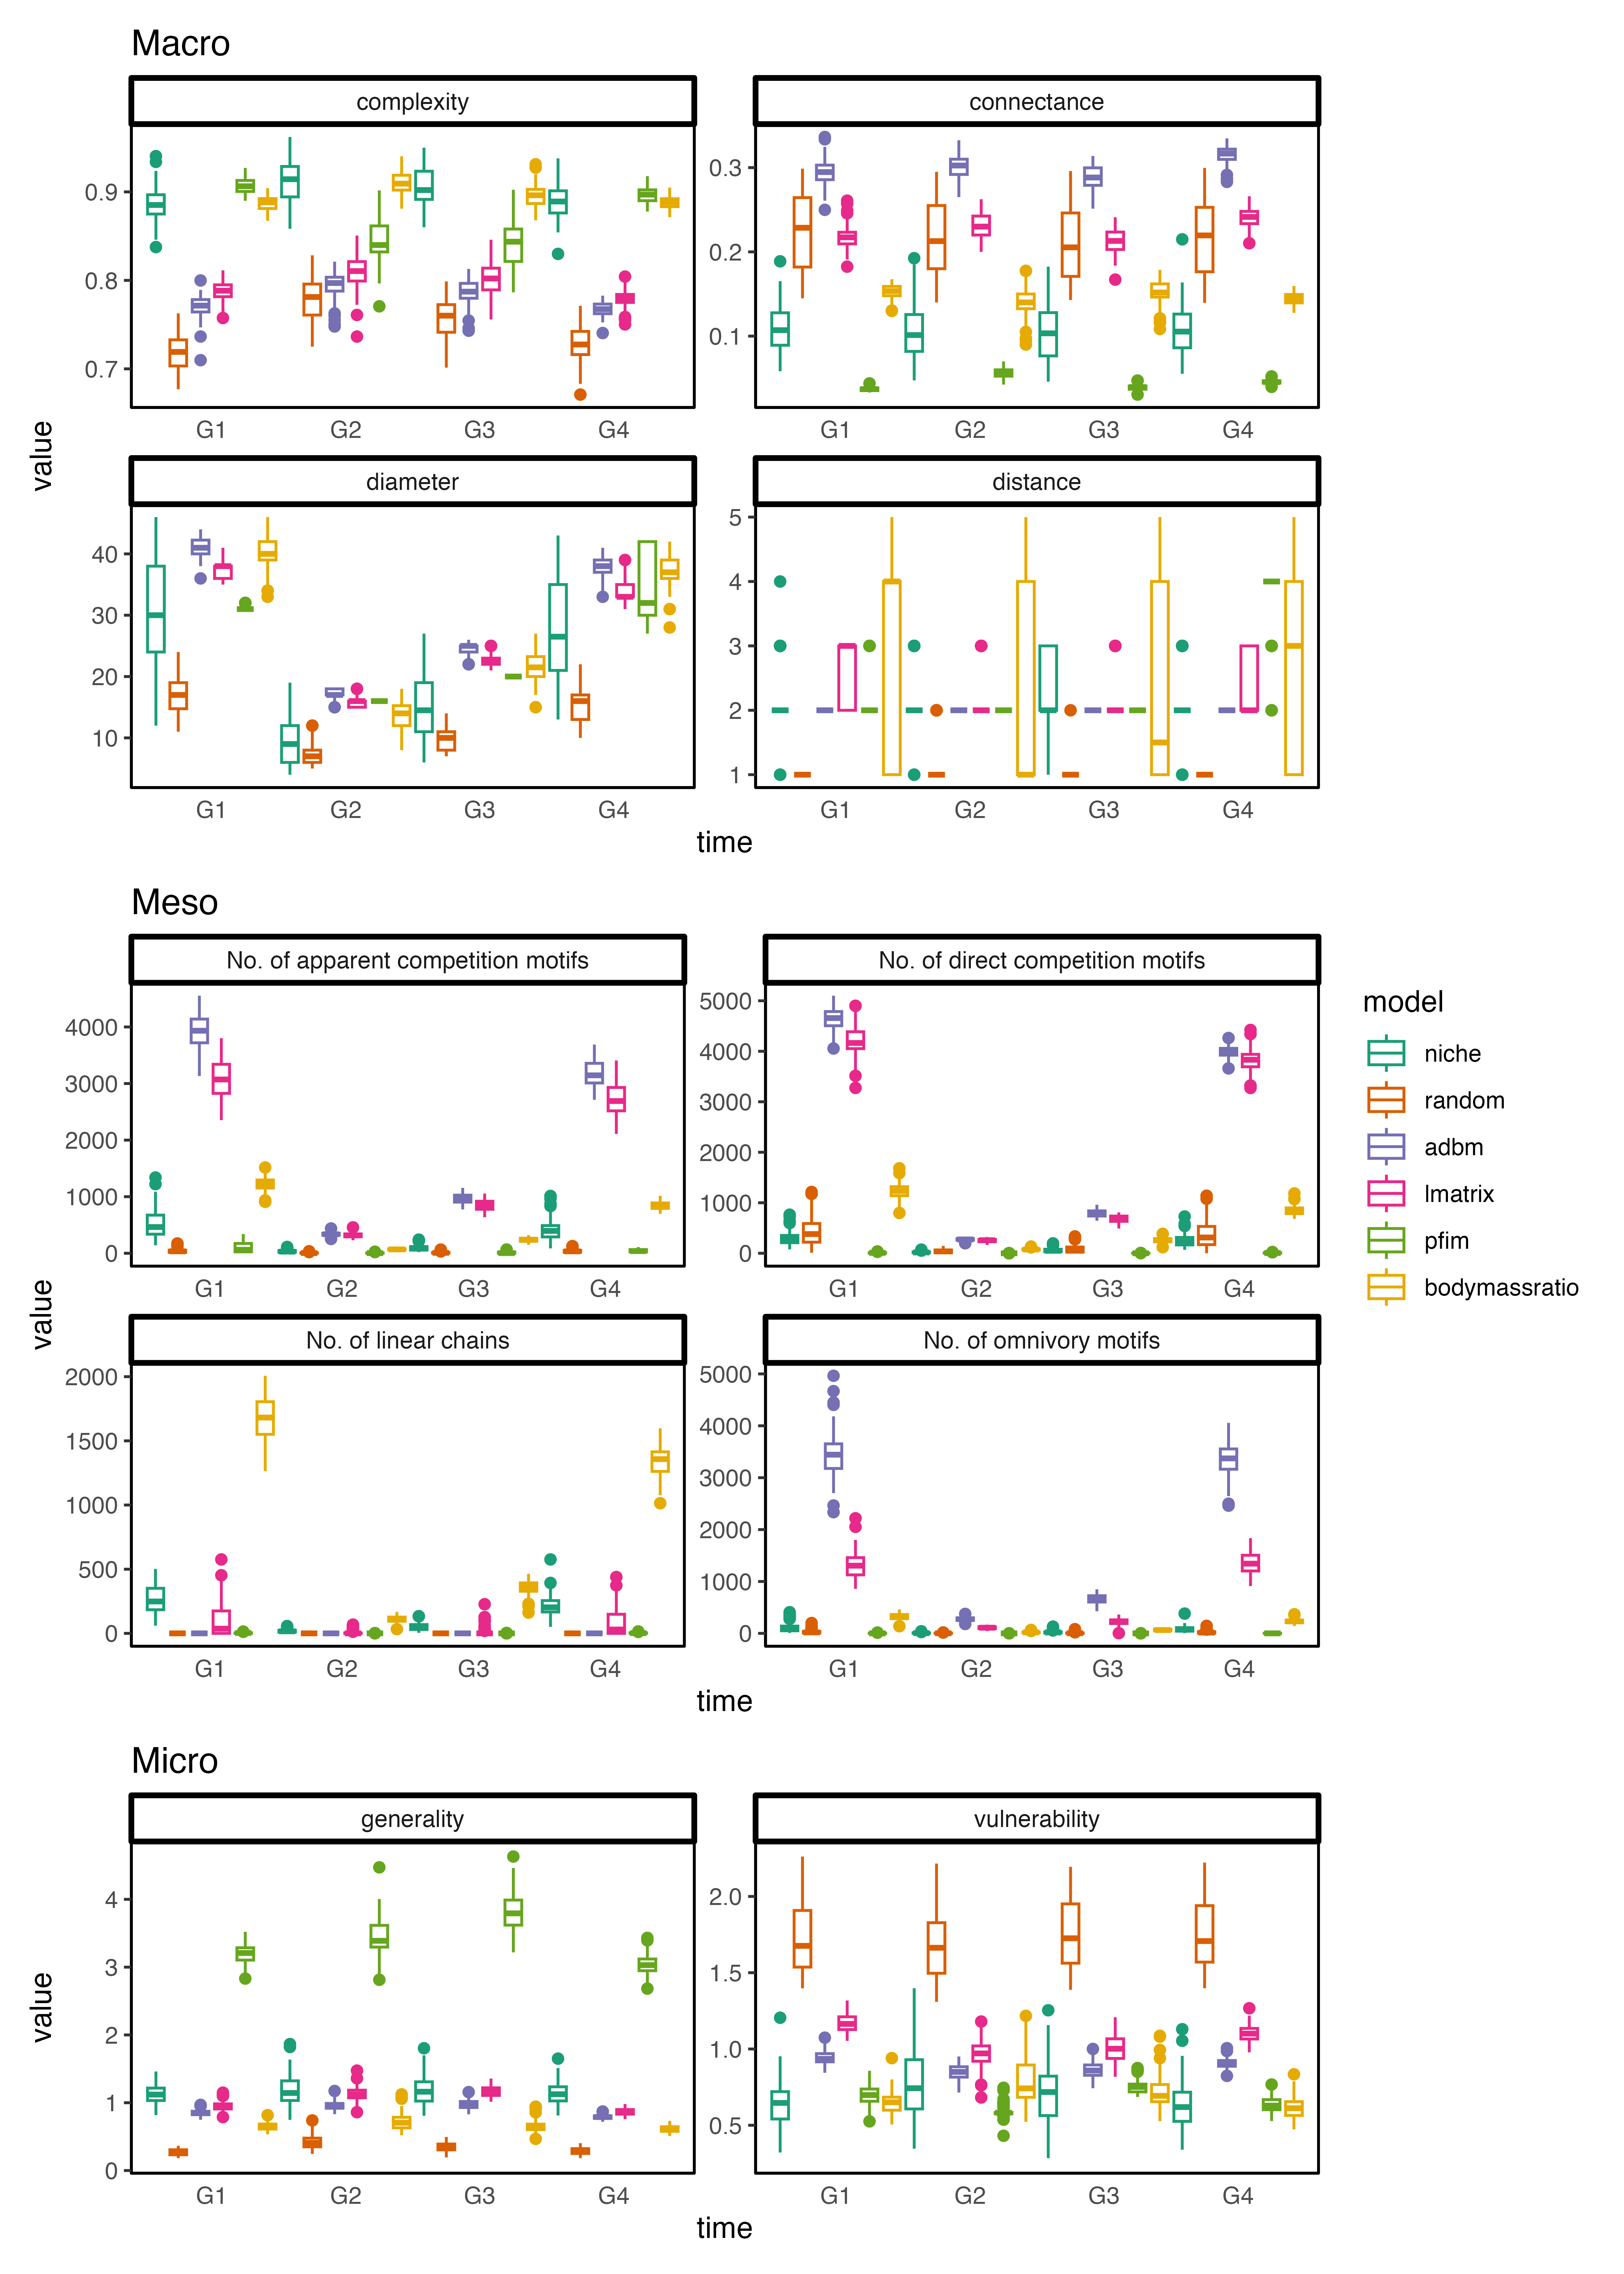
\includegraphics[keepaspectratio]{figures/summary.png}}

}

\caption{\label{fig-summary}stuff\ldots{}}

\end{figure}%

\subsubsection{Interaction/species
turnover}\label{interactionspecies-turnover}

\begin{figure}

\centering{

\pandocbounded{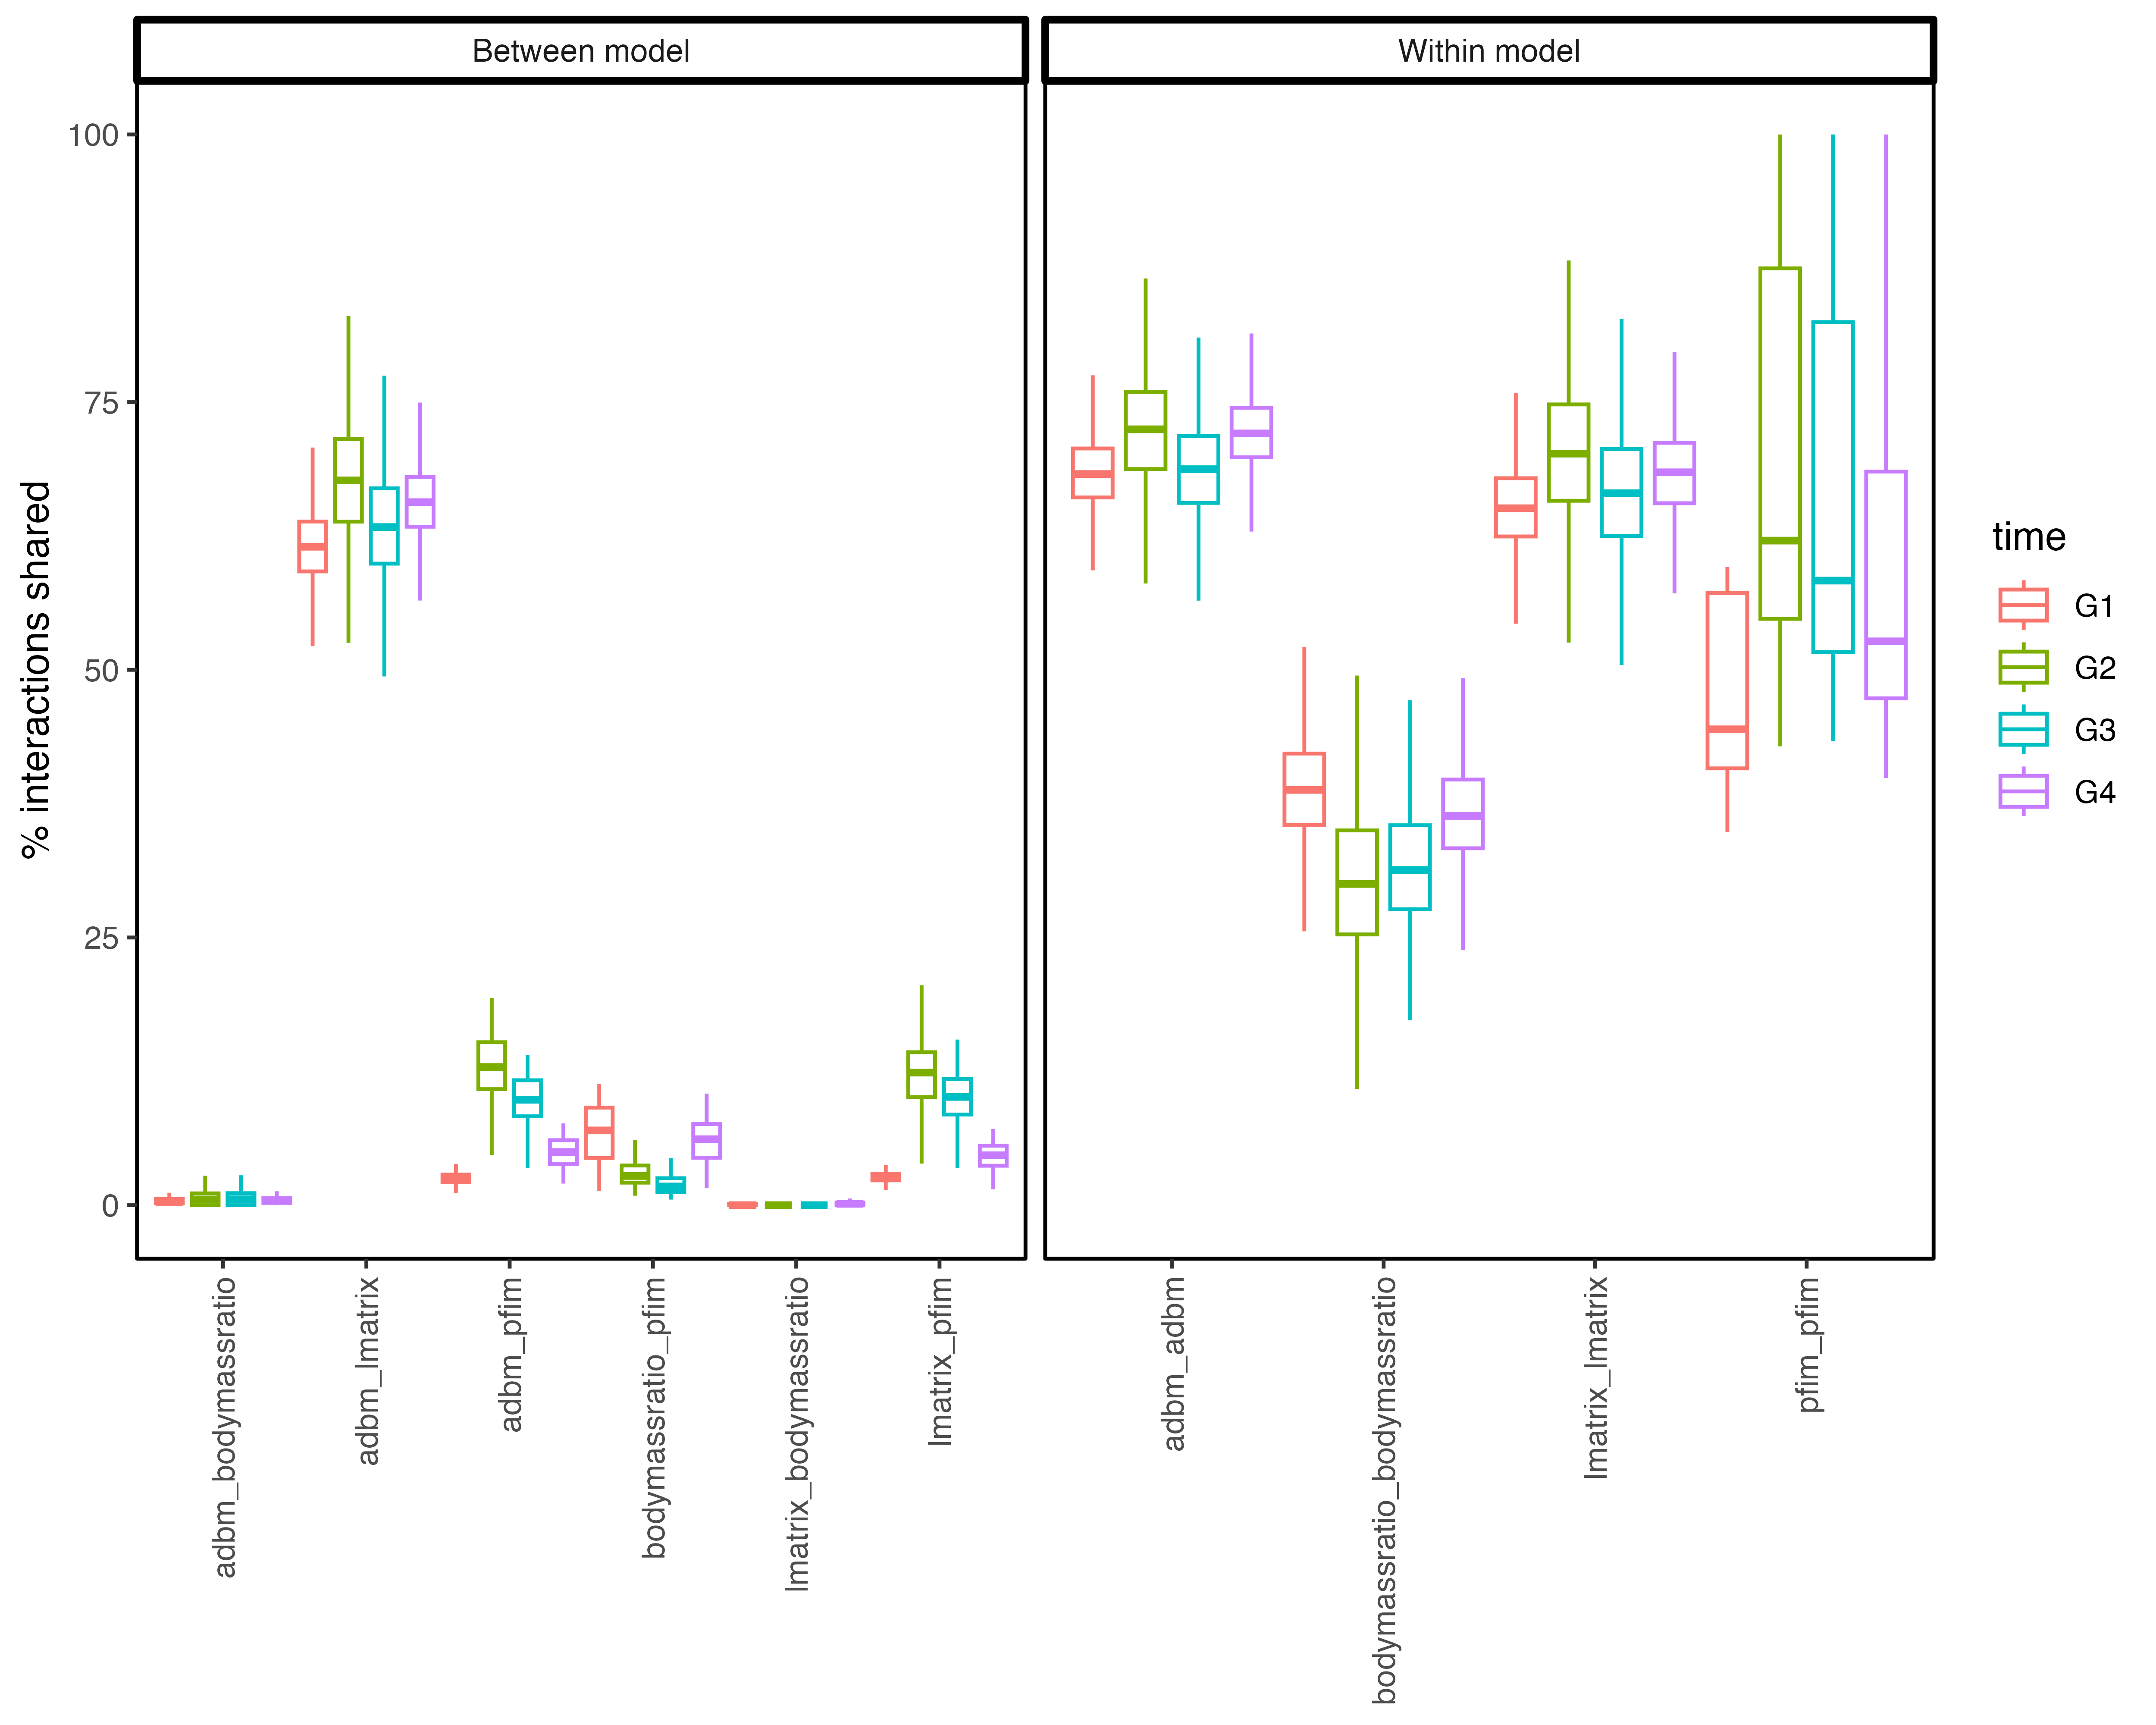
\includegraphics[keepaspectratio]{figures/beta_div.png}}

}

\caption{\label{fig-beta_div}stuff\ldots{} \% interaction shared is
calculated as number shared interactions / ((number interactions left -
shared interactions) + (number interactions right - shared interactions)
+ shared interactions). Additionally niche and random models are
excluded as it is illogical since both of these models are fundamentally
species agnostic}

\end{figure}%

\subsection{Comparing inference}\label{comparing-inference}

\begin{figure}

\centering{

\pandocbounded{\includegraphics[keepaspectratio]{figures/dunhill_comp.png}}

}

\caption{\label{fig-dunhill}stuff\ldots{} Recreation of the figure from
Dunhill 2024. Note not 100\% sold on the TSS and absolute mean
calculations\ldots{}}

\end{figure}%

\section*{References}\label{references}
\addcontentsline{toc}{section}{References}

\phantomsection\label{refs}
\begin{CSLReferences}{1}{0}
\bibitem[\citeproctext]{ref-allesina2008}
Allesina, S., Alonso, D., \& Pascual, M. (2008). A general model for
food web structure. \emph{Science}, \emph{320}(5876), 658--661.
\url{https://doi.org/10.1126/science.1156269}

\bibitem[\citeproctext]{ref-bambach2007}
Bambach, R. K., Bush, A. M., \& Erwin, D. H. (2007). Autecology and the
Filling of Ecospace: Key Metazoan Radiations. \emph{Palaeontology},
\emph{50}(1), 1--22.
\url{https://doi.org/10.1111/j.1475-4983.2006.00611.x}

\bibitem[\citeproctext]{ref-caron2022}
Caron, D., Maiorano, L., Thuiller, W., \& Pollock, L. J. (2022).
Addressing the Eltonian shortfall with trait-based interaction models.
\emph{Ecology Letters}, \emph{25}(4), 889--899.
\url{https://doi.org/10.1111/ele.13966}

\bibitem[\citeproctext]{ref-delmas2018}
Delmas, E., Besson, M., Brice, M.-H., Burkle, L. A., Dalla Riva, G. V.,
Fortin, M.-J., Gravel, D., Guimarães, P. R., Hembry, D. H., Newman, E.
A., Olesen, J. M., Pires, M. M., Yeakel, J. D., \& Poisot, T. (2018).
Analysing ecological networks of species interactions. \emph{Biological
Reviews}, 112540. \url{https://doi.org/10.1111/brv.12433}

\bibitem[\citeproctext]{ref-dunhill2024}
Dunhill, A. M., Zarzyczny, K., Shaw, J. O., Atkinson, J. W., Little, C.
T. S., \& Beckerman, A. P. (2024). Extinction cascades, community
collapse, and recovery across a Mesozoic hyperthermal event.
\emph{Nature Communications}, \emph{15}(1), 8599.
\url{https://doi.org/10.1038/s41467-024-53000-2}

\bibitem[\citeproctext]{ref-dunne2014}
Dunne, J. A., Labandeira, C. C., \& Williams, R. J. (2014). Highly
resolved early eocene food webs show development of modern trophic
structure after the end-cretaceous extinction. \emph{Proceedings of the
Royal Society B: Biological Sciences}, \emph{281}(1782), 20133280.
\url{https://doi.org/10.1098/rspb.2013.3280}

\bibitem[\citeproctext]{ref-erdos1959}
Erdős, P., \& Rényi, A. (1959). On random graphs. i. \emph{Publicationes
Mathematicae Debrecen}, \emph{6}(3-4), 290--297.
\url{https://doi.org/10.5486/pmd.1959.6.3-4.12}

\bibitem[\citeproctext]{ref-fricke2022}
Fricke, E. C., Hsieh, C., Middleton, O., Gorczynski, D., Cappello, C.
D., Sanisidro, O., Rowan, J., Svenning, J.-C., \& Beaudrot, L. (2022).
Collapse of terrestrial mammal food webs since the Late Pleistocene.
\emph{Science}, \emph{377}(6609), 1008--1011.
\url{https://doi.org/10.1126/science.abn4012}

\bibitem[\citeproctext]{ref-gauzens2023}
Gauzens, B., Brose, U., Delmas, E., \& Berti, E. (2023). ATNr:
Allometric Trophic Network models in R. \emph{Methods in Ecology and
Evolution}, \emph{14}(11), 2766--2773.
\url{https://doi.org/10.1111/2041-210X.14212}

\bibitem[\citeproctext]{ref-gupta2022}
Gupta, A., Furrer, R., \& Petchey, O. L. (2022). Simultaneously
estimating food web connectance and structure with uncertainty.
\emph{Ecology and Evolution}, \emph{12}(3), e8643.
\url{https://doi.org/10.1002/ece3.8643}

\bibitem[\citeproctext]{ref-jonsson2015}
Jonsson, T., Berg, S., Pimenov, A., Palmer, C., \& Emmerson, M. (2015).
The reliability of R50 as a measure of vulnerability of food webs to
sequential species deletions. \emph{Oikos}, \emph{124}(4), 446--457.
\url{https://doi.org/10.1111/oik.01588}

\bibitem[\citeproctext]{ref-martinez1992}
Martinez, N. D. (1992). Constant connectance in community food webs.
\emph{The American Naturalist}, \emph{139}(6), 1208--1218.
\url{http://www.jstor.org/stable/2462337}

\bibitem[\citeproctext]{ref-milo2002}
Milo, R., Shen-Orr, S., Itzkovitz, S., Kashtan, N., Chklovskii, D., \&
Alon, U. (2002). Network motifs: Simple building blocks of complex
networks. \emph{Science}, \emph{298}(5594), 824--827.
\url{https://doi.org/10.1126/science.298.5594.824}

\bibitem[\citeproctext]{ref-petchey2008}
Petchey, O. L., Beckerman, A. P., Riede, J. O., \& Warren, P. H. (2008).
Size, foraging, and food web structure. \emph{Proceedings of the
National Academy of Sciences}, \emph{105}(11), 4191--4196.
\url{https://doi.org/10.1073/pnas.0710672105}

\bibitem[\citeproctext]{ref-poisot2012}
Poisot, T., Canard, E., Mouquet, N., \& Hochberg, M. E. (2012). A
comparative study of ecological specialization estimators. \emph{Methods
in Ecology and Evolution}, \emph{3}(3), 537--544.
\url{https://doi.org/10.1111/j.2041-210x.2011.00174.x}

\bibitem[\citeproctext]{ref-rohr2010}
Rohr, R., Scherer, H., Kehrli, P., Mazza, C., \& Bersier, L.-F. (2010).
Modeling food webs: Exploring unexplained structure using latent traits.
\emph{The American Naturalist}, \emph{176}(2), 170--177.
\url{https://doi.org/10.1086/653667}

\bibitem[\citeproctext]{ref-roopnarine2006}
Roopnarine, P. D. (2006). Extinction cascades and catastrophe in ancient
food webs. \emph{Paleobiology}, \emph{32}(1), 1--19.
\url{https://www.jstor.org/stable/4096814}

\bibitem[\citeproctext]{ref-roopnarine2017}
Roopnarine, P. D. (2017). \emph{Ecological Modelling of Paleocommunity
Food Webs} (pp. 201--226). University of Chicago Press.

\bibitem[\citeproctext]{ref-schneider2016}
Schneider, F. D., Brose, U., Rall, B. C., \& Guill, C. (2016). Animal
diversity and ecosystem functioning in dynamic food webs. \emph{Nature
Communications}, \emph{7}(1), 12718.
\url{https://doi.org/10.1038/ncomms12718}

\bibitem[\citeproctext]{ref-schoener1989}
Schoener, T. W. (1989). Food Webs From the Small to the Large: The
Robert H. MacArthur Award Lecture. \emph{Ecology}, \emph{70}(6),
1559--1589. \url{https://doi.org/10.2307/1938088}

\bibitem[\citeproctext]{ref-shaw2024}
Shaw, J. O., Dunhill, A. M., Beckerman, A. P., Dunne, J. A., \& Hull, P.
M. (2024). \emph{A framework for reconstructing ancient food webs using
functional trait data} (p. 2024.01.30.578036). bioRxiv.
\url{https://doi.org/10.1101/2024.01.30.578036}

\bibitem[\citeproctext]{ref-staniczenko2013}
Staniczenko, P. P. A., Kopp, J. C., \& Allesina, S. (2013). The ghost of
nestedness in ecological networks. \emph{Nature Communications},
\emph{4}(1), 1391. \url{https://doi.org/10.1038/ncomms2422}

\bibitem[\citeproctext]{ref-stouffer2007}
Stouffer, D. B., Camacho, J., Jiang, W., \& Nunes Amaral, L. A. (2007).
Evidence for the existence of a robust pattern of prey selection in food
webs. \emph{Proceedings of the Royal Society B: Biological Sciences},
\emph{274}(1621), 1931--1940.
\url{https://doi.org/10.1098/rspb.2007.0571}

\bibitem[\citeproctext]{ref-strydom2023}
Strydom, T., Bouskila, S., Banville, F., Barros, C., Caron, D., Farrell,
M. J., Fortin, M.-J., Mercier, B., Pollock, L. J., Runghen, R., Dalla
Riva, G. V., \& Poisot, T. (2023). Graph embedding and transfer learning
can help predict potential species interaction networks despite data
limitations. \emph{Methods in Ecology and Evolution}, \emph{14}(12),
2917--2930. \url{https://doi.org/10.1111/2041-210X.14228}

\bibitem[\citeproctext]{ref-strydom2021b}
Strydom, T., Catchen, M. D., Banville, F., Caron, D., Dansereau, G.,
Desjardins-Proulx, P., Forero-Muñoz, N. R., Higino, G., Mercier, B.,
Gonzalez, A., Gravel, D., Pollock, L., \& Poisot, T. (2021). A roadmap
towards predicting species interaction networks (across space and time).
\emph{Philosophical Transactions of the Royal Society B: Biological
Sciences}, \emph{376}(1837), 20210063.
\url{https://doi.org/10.1098/rstb.2021.0063}

\bibitem[\citeproctext]{ref-strydom2021}
Strydom, T., Dalla Riva, G. V., \& Poisot, T. (2021). SVD entropy
reveals the high complexity of ecological networks. \emph{Frontiers in
Ecology and Evolution}, \emph{9}.
\url{https://doi.org/10.3389/fevo.2021.623141}

\bibitem[\citeproctext]{ref-williams2000}
Williams, R. J., \& Martinez, N. D. (2000). Simple rules yield complex
food webs. \emph{Nature}, \emph{404}(6774), 180--183.
\url{https://doi.org/10.1038/35004572}

\bibitem[\citeproctext]{ref-williams2004}
Williams, R. J., \& Martinez, N. D. (2004). Stabilization of chaotic and
non-permanent food-web dynamics. \emph{The European Physical Journal B -
Condensed Matter}, \emph{38}(2), 297--303.
\url{https://doi.org/10.1140/epjb/e2004-00122-1}

\bibitem[\citeproctext]{ref-williams2008}
Williams, R. J., \& Martinez, N. D. (2008). Success and its limits among
structural models of complex food webs. \emph{The Journal of Animal
Ecology}, \emph{77}(3), 512--519.
\url{https://doi.org/10.1111/j.1365-2656.2008.01362.x}

\bibitem[\citeproctext]{ref-yeakel2014}
Yeakel, J. D., Pires, M. M., Rudolf, L., Dominy, N. J., Koch, P. L.,
Guimarães, P. R., \& Gross, T. (2014). Collapse of an ecological network
in ancient egypt. \emph{PNAS}, \emph{111}(40), 14472--14477.
\url{https://doi.org/10.1073/pnas.1408471111}

\end{CSLReferences}





\end{document}
